In regards to experiments and results, it is essential to address the impact of using a sigmoid activation in the final layer and normalizing the data after being fit into the model. These factors have led to suboptimal model training, despite initial expectations. Consequently, the decision has been made to split the experiments and results section into two parts. Initially, the focus will be on hyperparameter decisions and comparisons across various datasets and metrics. For those models that were able to be retrained enough to display the metrics correctly and see their comparisons, the table has been changed. Subsequently, a separate section will present the results obtained with the current models, highlighting their limitations and proposing potential solutions to address these issues.

\subsection{Challenges with data normalization}
Normalizing data is a crucial step in data preprocessing, especially in the context of computer vision, when it is useful to know the imagery mean and deviation. It ensures that data is consistent across the dataset, making it easier to compare and analyze different data points. Many optimizers converge faster when data is normalized, as it ensures features have similar scales, making optimization landscapes more symmetric.
\\
\\
In this case, the data exhibited a wide range from 0 to 10,000. At that time, it was strongly emphasized that this preprocessing step was vital because excessively preprocessing the cloud-free and cloud-covered images could result in an unrealistic model. To address this concern, normalizing the data was considered. Nevertheless, performing min-max scaling did not yield favorable outcomes for several reasons:
\begin{itemize}
	\item The output data values became very constrained, preventing neural networks from making substantial adjustments, resulting in a persistently low function loss. 
	\item It was expected that metrics like \gls{mse}, and \gls{mae} would register smaller values due to the scaling. However, it was not anticipated that the parameters \gls{ssim} metric should also be changed. This implies that achieving an \gls{ssim} metric around 1 with such small output values is not equivalent to achieving the same \gls{ssim} if the data range is not checked. Applying these metrics in such a small range has meant that they cannot provide enough information to the models.
\end{itemize}
At this point, it became apparent that utilizing the sigmoid function plus the normalization was not as effective as initially thought. Due to the wide range of values, applying normalization did not significantly impact the loss function, specifically in this case, the \gls{mse} score, when dealing with very small differences once the training had already taken some epochs. After addressing the issue, two methods for preventing this problem have been identified:
\begin{itemize}
	\item Clipping: This method involves limiting the range of values in an image. In \cite{Meraner2020}, they employ clipping to constrain the values within the range of 0 to 2000.
	\item Scaling Sigmoid Activation: It is indeed advantageous to use a sigmoid activation as the final function since it constrains the neural network's output. Instead of removing the sigmoid, it is recommended to keep it and adjust its final output value by scaling it according to the range of values present in the dataset.
\end{itemize}
Both options can be implemented concurrently. Nevertheless, the decision between utilizing clipping or employing a sigmoid has been deferred to future iterations of the project.
\subsection{Results}
To start this section, we will address the issue of underfitting. To observe the progression of the networks, we initially employed simpler models, such as \texttt{Carla} or \texttt{Anna}. Subsequently, we incorporated similar structures and introduced new ones, gradually increasing the complexity, as seen in the \texttt{Regina} and \texttt{Ausias} models, respectively.
\\
\\
Regarding the \texttt{Carla} model, it is evident that it lacks the capacity to further minimize its loss function. Also, there are instances when the validation dataset exhibits slight fluctuations. This is a clear case of underfitting. The occurrence of underfitting as early as the first epoch is primarily attributed to the use of a very low batch size. A smaller batch size implies that the model is processing more precise but limited information at each step, leading to a more optimized backpropagation of tensors for each individual case.
\begin{figure}[H]
	\centering
	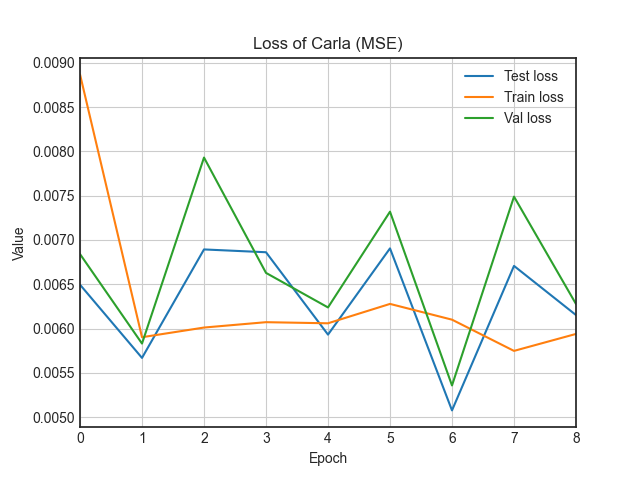
\includegraphics[width=10cm]{imgs/models/models/cnn/loss.png}
	\caption{Loss of the Carla best run.}
	\label{fig:models-carla-loss}
\end{figure}
When it comes to the utilization of residual blocks, there is a significant difference in the loss between \texttt{Carla} and \texttt{Regina} in Figure \ref{tab:models-metrics-cnn}, despite the fact that the normalized values are not accurate.
\begin{table}[H]
	\caption{Comparison of metrics between \texttt{Carla} and original \texttt{Regina} (with data normalization)}
	\centering
	\begin{tabular}{lcc}
		Model  &  MSE  & PSNR  \\ \hline
		Regina & 0.252 & 27.57 \\
		Carla  & 0.603 & 10.21
	\end{tabular}
	\label{tab:models-metrics-cnn}
\end{table}
The table \ref{tab:models-metrics-regina} demonstrates that \gls{sar} data has substantial impact on the metrics, making them slightly more challenging. On the other hand, using data augmentation does not improve significantly the scores. This marginal changes in augmenting the data could be attributed to the dataset's inherent variability, which allows for the detection of complex correlations between the spectral bands. Although the augmented data was about 30 \%, it seems it does not incorporate value to the dataset.
\begin{table}[H]
	\caption{Comparison of metrics between variants of \texttt{Regina} (with normalized data).}
	\centering
	\begin{tabular}{ll|ccc}
		SAR & Augmented &  MSE  & PSNR  & SSIM  \\ \hline
		No  & No        & 0.23  & 6.38  & 0.15  \\
		No  & Yes       & 0.15  & 9.28  & 0.10  \\
		Yes & No        & 0.002 & 27.57 & 0.783 \\
		Yes & Yes       & 0.005 & 23.01 & 0.32
	\end{tabular}
	\label{tab:models-metrics-regina}
\end{table}
It is noteworthy that the \texttt{Anna} and \texttt{Veronica} models, which involve the transition from 2D data to 1D data and then back to 2D, encounter greater difficulty in establishing correlations among their neurons. Conversely, models that incorporate a bottleneck but maintain the data in a 2D format do not experience as much difficulty during training. Additionally, to further enhance the Ausias model, a convolutional layer was integrated after each de-convolution, serving as an analogy to process these layers and unify different kernels generated based on input values.
 In the end, the model known as AusiasConv emerged as the top-performing autoencoder within its category.
\begin{table}[H]
	\caption{Comparison of metrics of the autoencoders (without normalizing data).}
	\centering
	\begin{tabular}{l|cccl}
		Model               &       MSE        &      PSNR       &     SSIM      & CARL            \\ \hline
		Veronica            &      69285       &      -0.32      &     -3.93     & 4354.43         \\
		Anna                &      64432       &      0.04       &     -1.93     & 3320.87         \\
		AnnaSkip            &      27430       &      2.443      &     -1.32     & 954.32          \\
		Ausias              &     9423.32      &      8.38       &     0.01      & \textbf{293.32} \\
		\textbf{AusiasConv} & \textbf{6485.80} & \textbf{10.011} & \textbf{0.08} & 302.88
	\end{tabular}
	\label{tab:models-metrics-ae}
\end{table}
Furthermore, a training comparison was conducted using both the \gls{mse} and \gls{mae} loss functions, as the calculation methods for these results share significant similarities. It can be observed in \ref{tab:models-l1} that models trained with the \gls{mae} loss function yielded poorer results and exhibited considerably more instability compared to those trained with MSE, since the model weights were far more inbalanced and they could output \texttt{NaN}s results.
\begin{figure}[H]
\centering
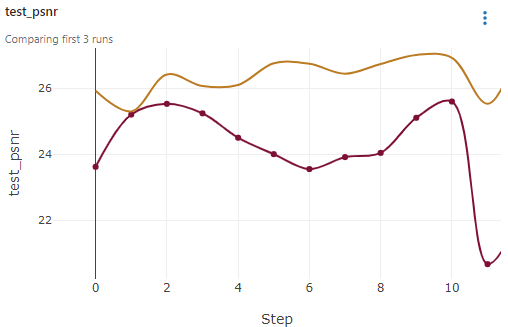
\includegraphics[width=12cm]{imgs/models/ausiasconvl1.png}
\caption{Comparison of test PSNR with L1 (red) and MSE (orange) of AusiasConv, normalized data.}
\label{fig:models-carla-loss}
\end{figure}
\begin{table}[H]
	\caption{Comparison of loss functions in Ausias model (normalized data).}
	\centering
	\begin{tabular}{ll|ccc}
		Model               & Loss Function &       MSE        &      PSNR       &      SSIM      \\ \hline
		AusiasConv          & L1            &     0.0058      & 22.3 &     -2.3      \\ %orderly-crab
		\textbf{AusiasConv} & MSE           & \textbf{0.003} & \textbf{25.22} & \textbf{ 0.08}
	\end{tabular}
	\label{tab:models-l1}
\end{table}
Regarding GAN training, while designing the discriminator's architecture presented challenges, the most demanding aspect was fine-tuning the hyperparameters to strike a balance between the two models in this adversarial setup. Initially, it was found that when using Adam as the optimizer, the beta values needed to be adjusted differently compared to a basic classification challenge scenario. Furthermore, the learning rate of the discriminator was lowered to minimize its learning during the initial iterations. Consequently, the weight decay for the discriminator was increased slightly to counteract its growing ability to detect changes in the generator.
\begin{table}[H]
	\centering
	\caption{Hyper parameters of RegiGAN}
	\begin{tabular}{l|cc}
		Hyper-parameter & Generator & Discriminator\\\hline
		Optimizer & Adam & Adam\\
		Learning rate & $10^-5$ & $10^-8$\\
		Weight decay & $5 \cdot 10^-5$ & $1 \cdot 10^-4$\\
		Beta A & 0.5  & 0.5\\
		Beta B & 0.999 & 0.999
	\end{tabular}
\end{table} 
Additionally, to assess the dynamics between the two networks, various parameters were introduced, including the accuracy of the discriminator, which ideally should hover around 0.5, and the scores for fake and real inputs, where both scores should also aim for 0.5. The "fake score" and the "real score" are terms commonly used in the context of \gls{gan} to assess the discriminator's performance. These scores represent how well the discriminator distinguishes between real and fake data samples during the training process. The real score is the output of the discriminator when it evaluates real data samples from the training dataset. Conversely, the fake score represents the output of the discriminator when it assesses generated (fake) data samples produced by the generator. These metrics played a crucial role in stabilizing the model. Actually, this metrics needed to be calculated in each batch, since any particular and remarkable change in the losses could led to desequilibrum.
\begin{figure}[H]
	\centering
	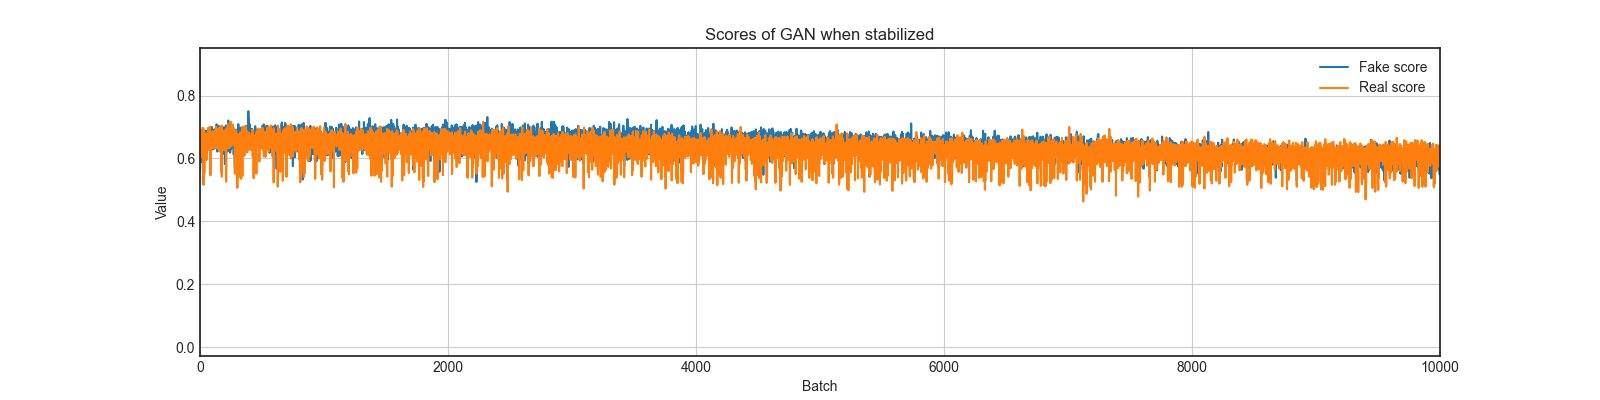
\includegraphics[width=16cm]{imgs/models/models/cnn/gan-score.png}
	\caption{Stabilized training}
	\label{fig:models-carla-loss}
\end{figure}
In the final stage, to assist the generative model in its initial iterations, the \gls{mse} loss function was introduced. This addition enabled the generative model to establish its bearings, enhance training stability, and maintain a clear focus on addressing the core problem.
\\
\\
It  can be seen in Figure \ref{fig:models-gan.mse} how the generator was able to perform better metrics than the \texttt{Regina}, although it is missing being able to see these metrics with the unnormalized data.
\begin{figure}[H]
	\centering
	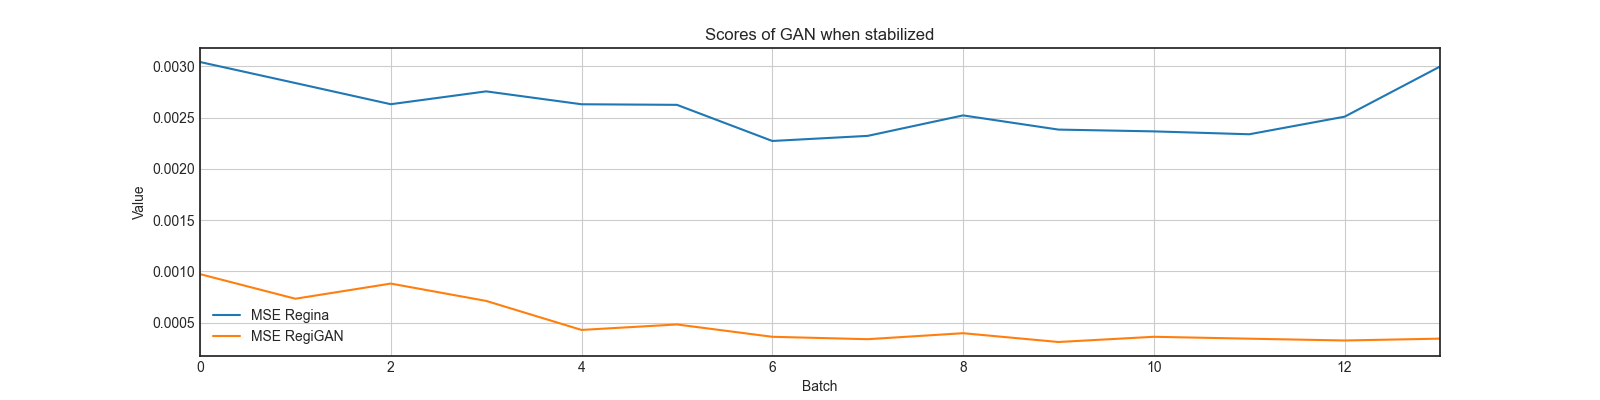
\includegraphics[width=16cm]{imgs/models/models/cnn/gan-mse.png}
	\caption{Comparison of MSE between RegiGAN and Regina.}
	\label{fig:models-gan.mse}
\end{figure}
\begin{table}[H]
	\caption{Comparison of loss functions between RegiGAN and Regina.}
	\centering
	\begin{tabular}{llcc}
		Model      & MSE              &  PSNR  &     SSIM      \\ \hline
		Regina     & \textbf{5867.52} & 10.60  & \textbf{0.49} \\
		AusiasConv & 6485.80          & 10.011 &     0.08
	\end{tabular}
	\label{tab:models-l1}
\end{table}
Regrettably, the diffusion model could not be deployed due to its prohibitively expensive training process and the inability to stabilize the model. Consequently, no metrics can be presented for the test data.
\begin{table}[H]
	\caption{Comparison of the scores of the models}
	\centering
	\begin{tabular}{llcc}
		Model                & MSE               &        PSNR        & SSIM  \\ \hline
		Regina    (ours)     & 5867.52           &       10.60        & 0.49  \\
		AusiasConv    (ours) & 6485.80           &       10.011       & 0.08  \\
		RegiGAN     (ours)   & 5863.467308044434 & 10.449258527964542 & 0.642 \\
		DSen2-CR             & -                 &       27.76        & 0.874 \\
		UnCRtainTS           & -                 &       28.90        & 0.88
	\end{tabular}
	\label{tab:models-l1}
\end{table}
In summary, this section sheds light on several crucial observations although the results are not quite good enough. Firstly, it becomes evident that transposed convolutions introduce a significant degree of imbalance into the network, resulting in training instability. Notably, the training of an image-to-image network presents a considerably higher level of imbalance compared to the more conventional tasks of classification or regression. This heightened imbalance necessitates a more pronounced fine-tuning process, a factor that was initially underestimated.
\\
\\
In general, it appears that the project may have not utilized sufficiently powerful neural networks. This decision was guided by the intention to proceed methodically and incrementally. Unfortunately, this cautious approach has resulted in delays. Consequently, there is a pressing need to consider the development of new models that are more aligned with achieving a practical solution.
\\
\\
The issue of normalization has exacerbated this situation. Regrettably, it was only recognized at a later stage that the models were not effectively learning, which contributed to the setbacks in the project's progress.
\\
\\
Furthermore, it becomes apparent that the utilization of autoencoders and \gls{vae} may have limitations when applied to larger images or when left in a latent space towards the end of the network architecture. It could be beneficial to explore alternative approaches, such as reconstructing images separately, one without clouds and another with clouds, to assess the network's behavior more effectively.
\\
\\
Additionally, there was an initial suspicion regarding the computational efficiency of diffusion models, but the extent of their time-consuming nature exceeded expectations, highlighting the need for careful consideration and optimization in their implementation.
\subsection{Experiments}
In this section, we will showcase the results of the top three models. Regrettably, due to normalization issues, we were unable to carry out tests involving bands 9. Furthermore, it's worth highlighting that both autoencoders and Variational Autoencoders (VAE) yielded unsatisfactory results. Consequently, displaying features and characteristics of the latent vector or the output image without achieving an accurate image reconstruction would not be meaningful.
\begin{table}[H]
	\caption{Comparison of the scores of the models}
	\centering
	\begin{tabular}{llcc}
		Model               & MSE              &      PSNR       &      SSIM      \\ \hline
		Regina           & 5867.52           &            10.60            & 0.49 \\
		AusiasConv & 6485.80 & 10.011 & 0.08\\
			RegiGAN             & 5863.467308044434       &     10.449258527964542      &     0.642      \\
	\end{tabular}
	\label{tab:models-l1}
\end{table}
To further analyze and compare the performance of the three leading models, a series of visualizations were carried out. It's interesting to note that \texttt{RegiGAN} doesn't excel in terms of metrics as \texttt{Regina} does, yet it demonstrates a noticeable advantage in image quality. This observation prompts two questions:
\begin{itemize}
	\item The consideration of a more robust loss function, as the current error approximation may not directly translate into qualitative enhancements.
	\item The possibility of errors in the metrics or image processing methods, which could be affecting the assessment of model performance.
\end{itemize}
Furthermore, it has been demonstrated that these models lack the necessary complexity and require additional training time, as the results obtained so far have not been satisfactory.
\begin{figure}[H]
	\centering
	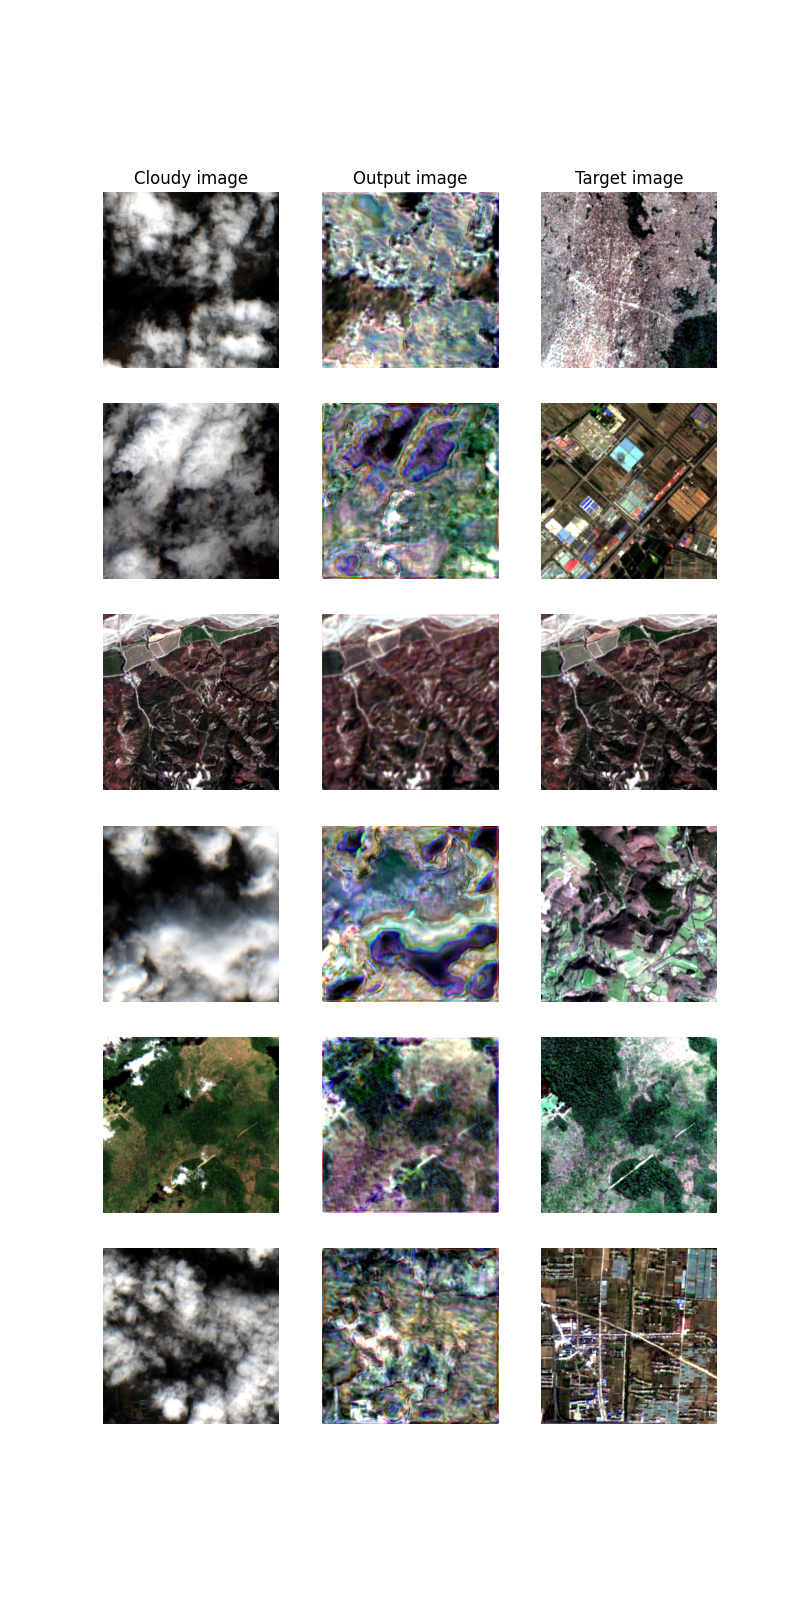
\includegraphics[width=10cm]{imgs/models/models/regina.png}
	\caption{Sample of cloudy (left) and cloudless (right) images along with \texttt{Regina}'s synthetic.}
	\label{fig:models-carla-loss}
\end{figure}
\begin{figure}[H]
	\centering
	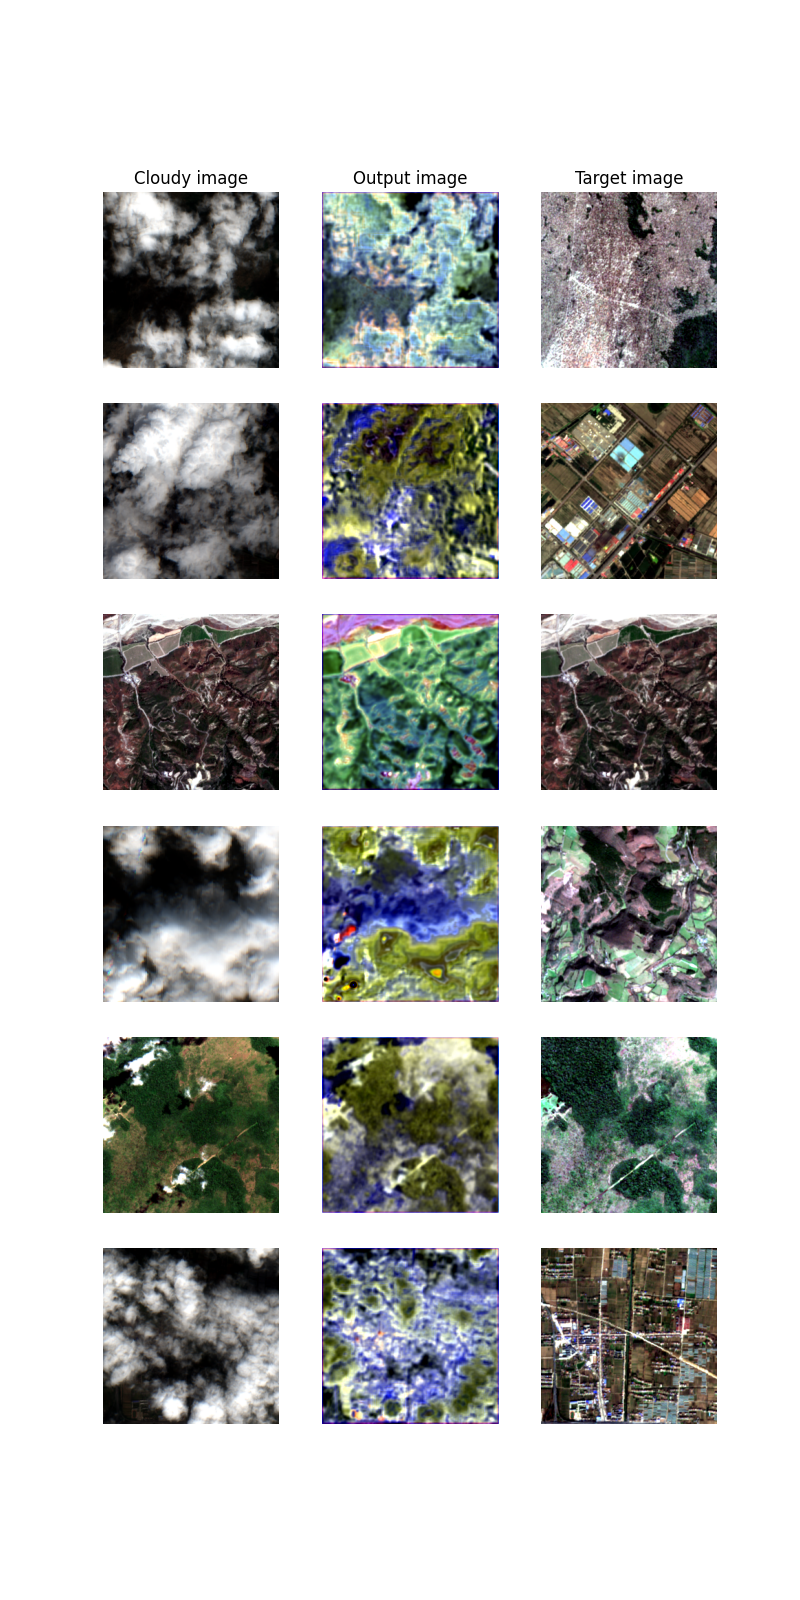
\includegraphics[width=10cm]{imgs/models/models/ausias.png}
	\caption{Sample of cloudy (left) and cloudless (right) images along with \texttt{Ausias}'s synthetic.}
	\label{fig:models-carla-loss}
\end{figure}
\begin{figure}[H]
	\centering
	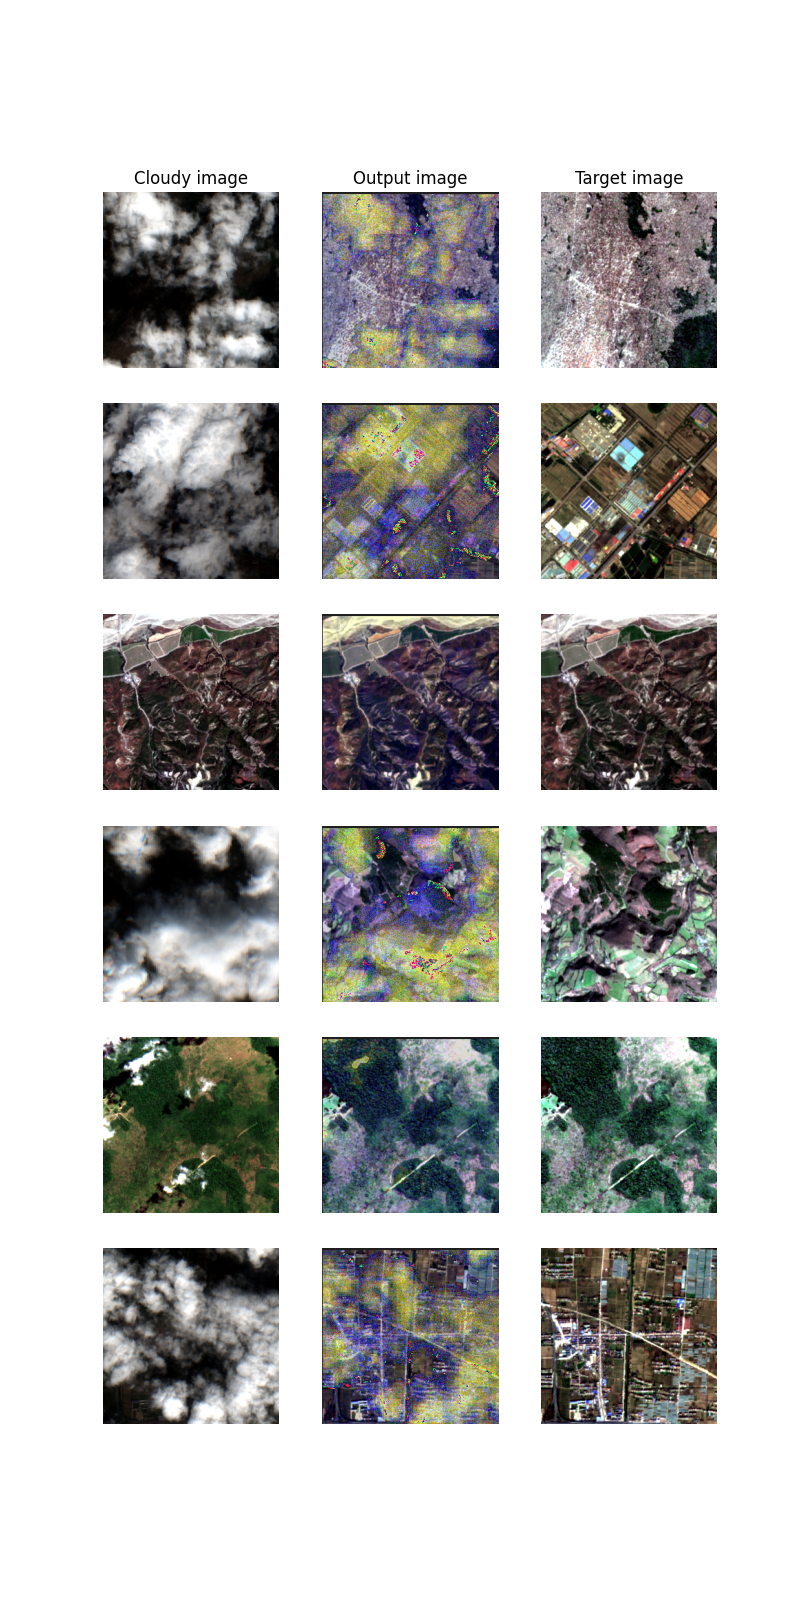
\includegraphics[width=10cm]{imgs/models/models/regigan.png}
	\caption{Sample of cloudy (left) and cloudless (right) images along with \texttt{RegiGAN}'s synthetic.}
	\label{fig:models-carla-loss}
\end{figure}

\section{Future directions}
The realm of generative modeling offers a vast spectrum of possibilities, and as exploration deepens, the horizons of what can be achieved continue to expand. Recognizing past challenges and learning from them will be crucial in charting the path forward.
\\
\\
A primary focus of the subsequent phase of this thesis will be to zero in on a singular network type. This decision emerges from the prior explorative phase, where various model architectures were extensively navigated. Concentrating on a specific network will allow for a more profound and nuanced understanding of its capabilities and limitations.
\\
\\
Furthermore, the choice of loss function is pivotal in the training process. The current losses, either due to their lack of specificity or computational intensity, may not be optimal. Future endeavors should emphasize identifying and implementing a more efficient and relevant loss function, ensuring not only enhanced training efficacy but also greater model precision.
\\
\\
Visualization plays an indispensable role in understanding the intricacies of data. A particularly intriguing observation was the significance of the ninth band in the reconstruction process. Delving deeper into such findings could unearth valuable insights and guide model refinement.
\\
\\
Lastly, as the project advances, leveraging the well-structured codebase will be advantageous. It would be prudent to add images in the a dedicated platform for training and tracking. The platform needs to facilitate real-time monitoring of the training process, enabling timely inferences from saved checkpoints.
\\
\\
In terms of visualizations and experiments, there has been lacking comparing models utilizing remote sensing with both real and synthetic images. This approach would allow us to assess whether it enhances the accuracy and effectiveness of the model.
\\
\\
In essence, as the future unfolds, a blend of specialization, efficient computational strategies, and insightful visual analyses will be paramount in propelling the research to new heights.
